 \section{凸包围体生成算法}

    \subsection{问题定义及算法流程}

     \frame{
       \frametitle{问题的定义}
      \begin{columns}[onlytextwidth]
          \begin{column}{0.7\textwidth}
           \begin{block}{凸包围~$k$~面体}%
            $k$-Convex Bounding Polyhedron,简称~$k$-CBP,可通过~$k$~个半空间定义:
              \begin{equation}
              \label{equ:kcbp_definition}
              \left\{
                \begin{array}{l}
                    k\mbox{-CBP} = \mathop  \bigcap \limits_{i = 1}^k \bm{H_i} \\
                    \bm{H_i} = \left\{ {\left. {\bm{p} \in {\mathbb{R}^3}} \right| \bm{n_i} \cdot \bm{p} \le {w_i}} , w_i \in \mathbb{R} \right\},
                \end{array}
              \right.
              \end{equation}
              其中,$\bm{n_i}$~是半空间~$\bm{H_i}$~的法向,方向指向包围体外部,
              $w_i$~是输入点集中沿~$\bm{n_i}$~方向投影的最大值。
           \end{block}
    %        \pgfputat{\pgfxy(5,0)}{\pgfbox[left,top]{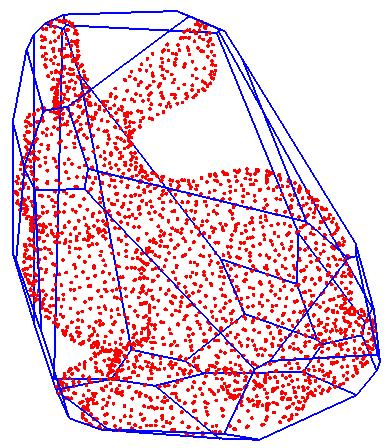
\includegraphics[width=0.25\textwidth]{bunny-34.png}}}
        \end{column}

       %\pgfputat{\pgfxy(7,-1.5)}{\pgfbox[left,top]{
       %  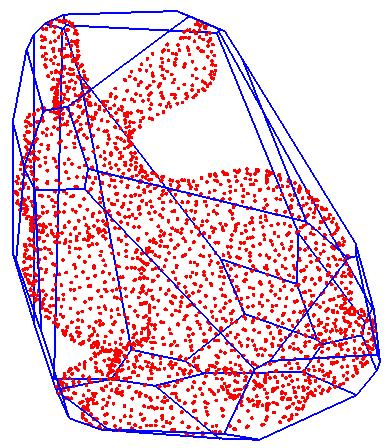
\includegraphics[width=0.25\textwidth]{bunny-34.png}
       %}}
        \begin{column}{0.4\textwidth}
        \begin{figure}
            %\pgfputat{\pgfxy(7,-1.5)}{\pgfbox[left,top]{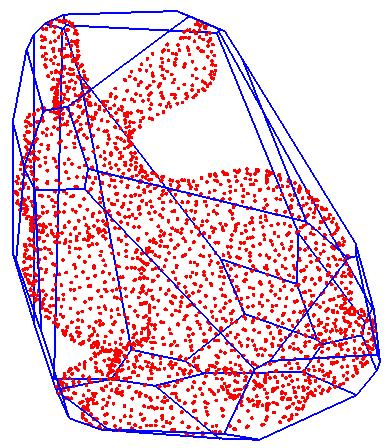
\includegraphics[width=0.8\textwidth]{bunny-34.png}}} %%cannot use caption for pgfputat
            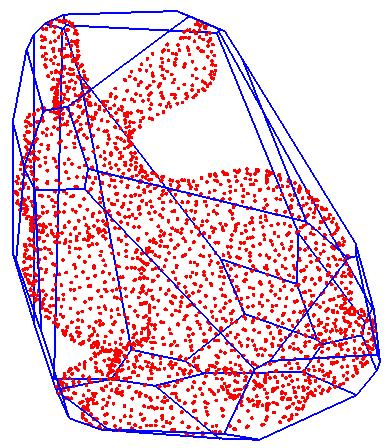
\includegraphics[width=0.8\textwidth]{bunny-34.png}
            \caption{34-CBP}
        \end{figure}
        \end{column}
      \end{columns}

      \note{这是凸包围多面体的定义,通俗些讲,其实就是空间中将模型包裹起来的k个平面,右图就是一个k=34的例子。
      其实这个问题的关键就是如何确定这些平面的方向。
      }
    }

       \frame{
       \frametitle{算法流程}
       \begin{block}{构造$k$-CBP~算法流程图}
        \begin{figure}
        \centering
        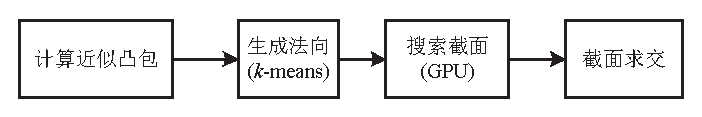
\includegraphics[width=4.0in]{kcbp-flowchart-x-aix.eps}
        \label{lbl:kcbp-algorithm-flowchart}
        \end{figure}
    \end{block}
    \begin{block}{关键步骤}
          \begin{description}
             \item[定法向:]结合近似内凸包和~$k$-means;
             \item[搜截面:]GPU~中沿各法向搜索切点构造截面;
             \item[求交点:]截面对偶映射求得交点。
          \end{description}
    \end{block}

    \note{这是本文构造凸包围多面体的算法流程图,关键就是这3步。\\
      定法向:方向的好坏直接决定最后多面体的紧致程度,本文结合了近似内凸包和kmeans聚类算法来确定法向。\\
      搜截面:因为法向确定后,搜索截面的过程各个法向之间相互独立互不影响,因此可以较方便用GPU加速。\\
      求交点:确定好平面后直接求交即可得到k-cbp的顶点。
    }
}

  \subsection{截面法向的生成}

    \frame{
        \frametitle{近似凸包的构造}
        \begin{figure}
        \vspace{-3mm}
        \subfloat[分组]
        {
           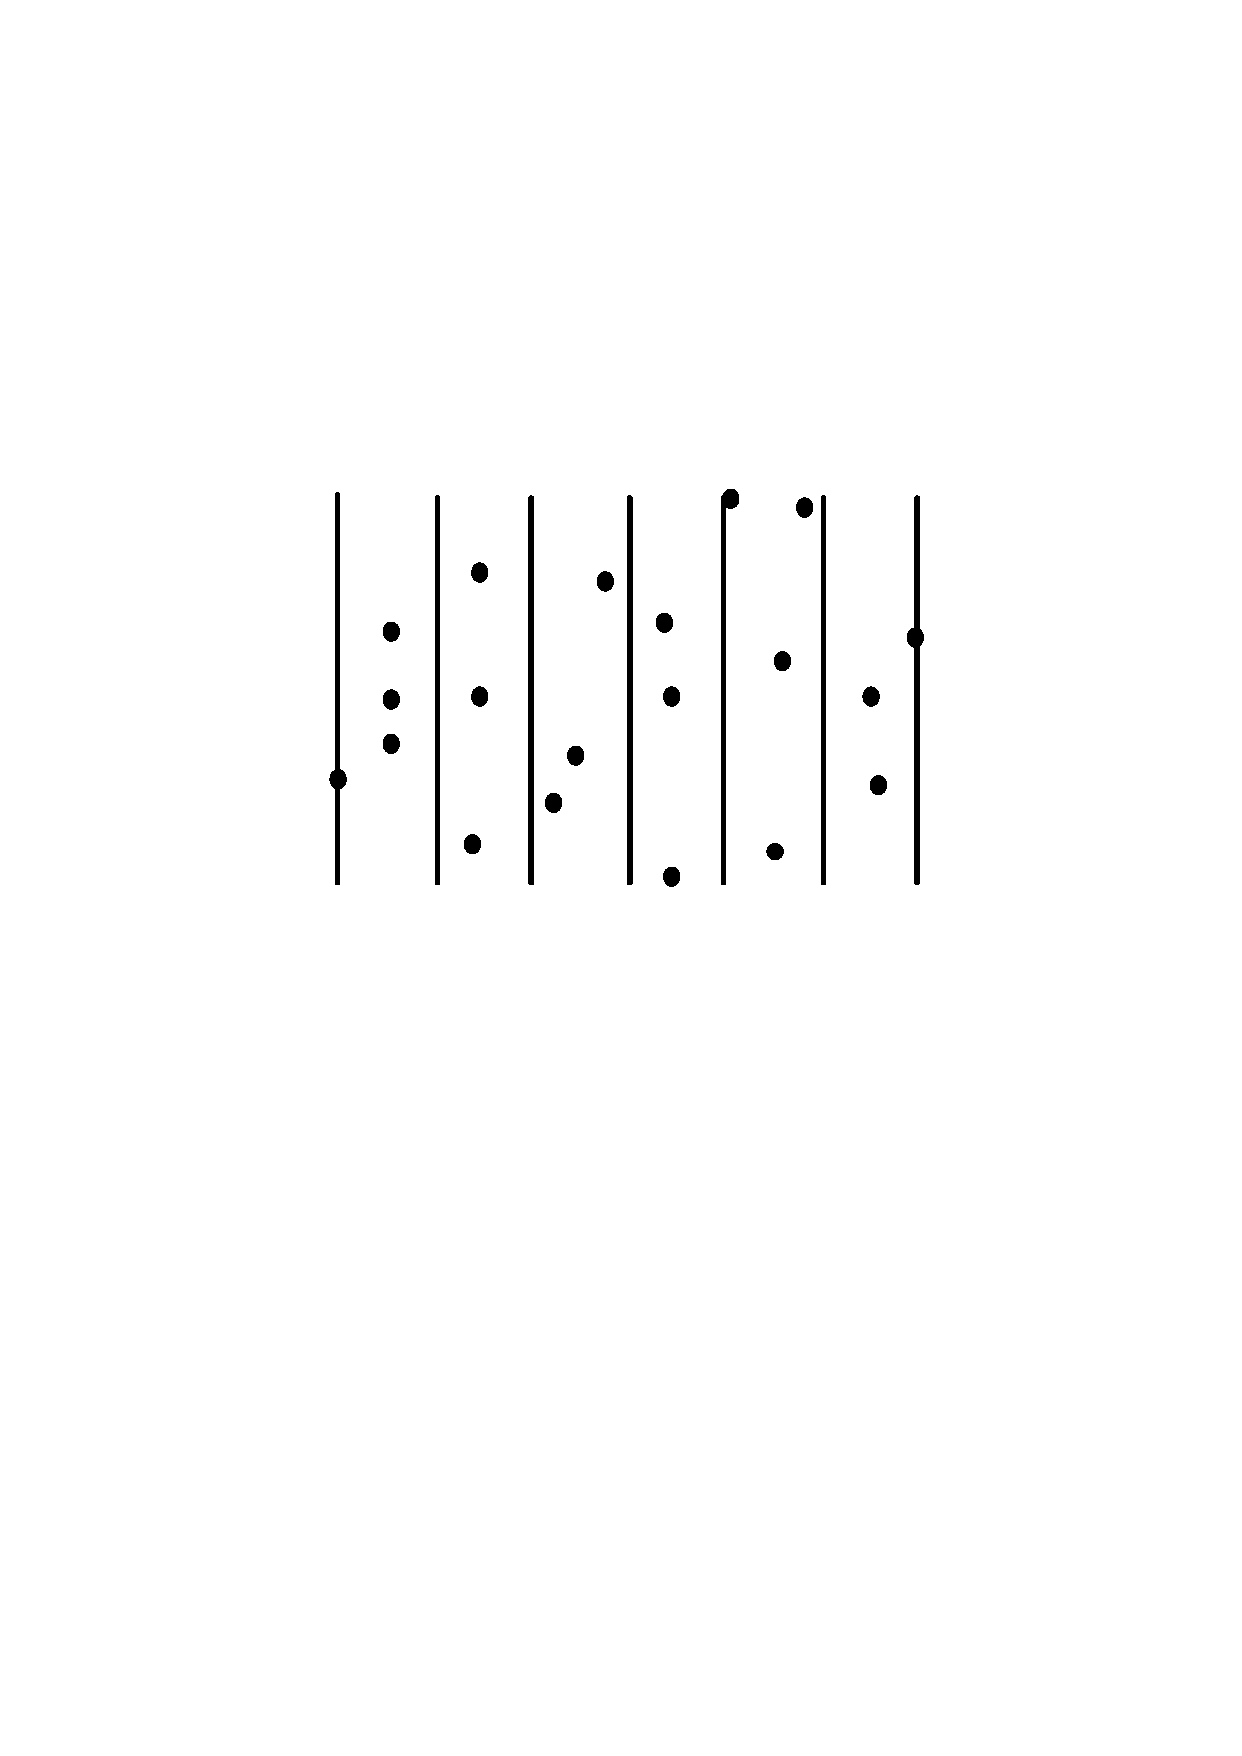
\includegraphics[width=0.28\textwidth]{figures/approximate-convexhull-step1.pdf}
        }\hspace{2mm}
        \subfloat[选极值点]
        {
            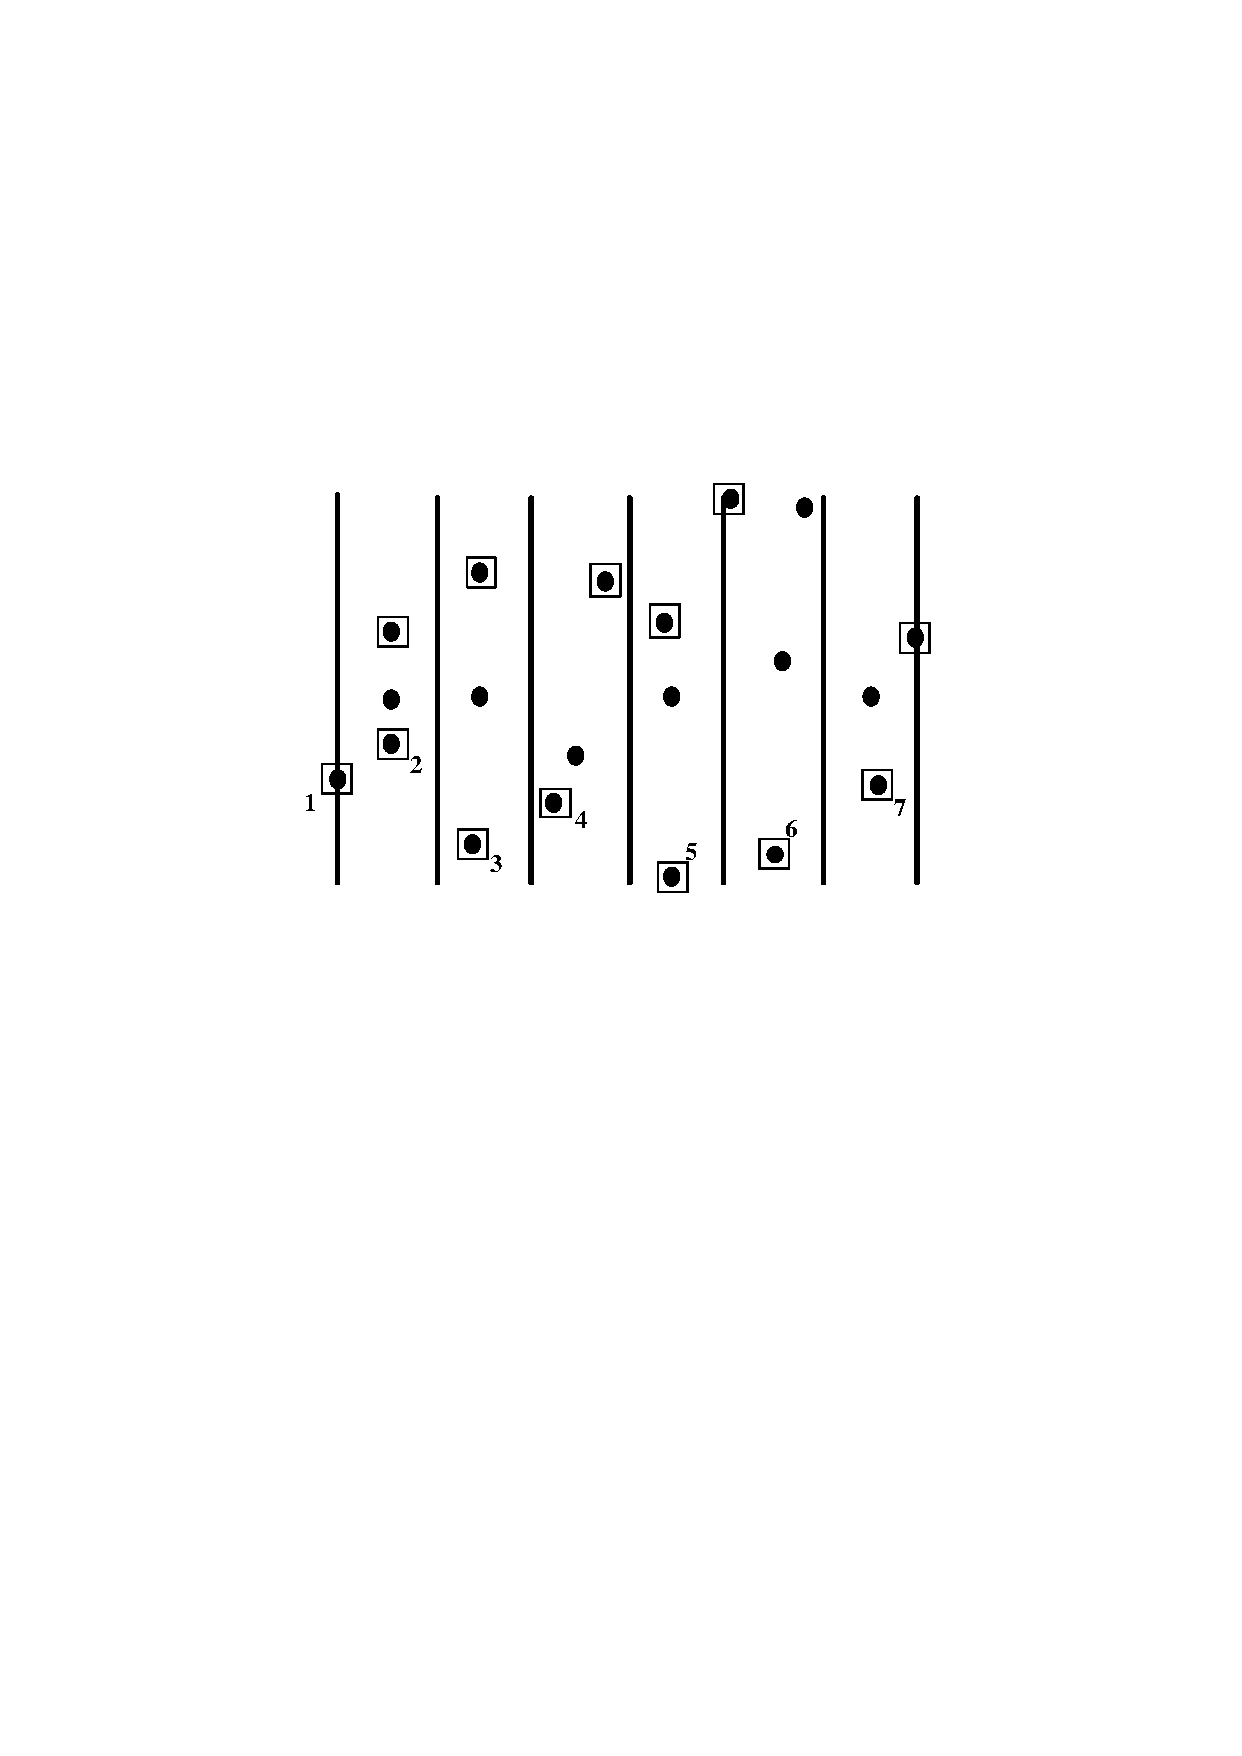
\includegraphics[width=0.28\textwidth]{figures/approximate-convexhull-step2.pdf}
        }\hspace{2mm}
        \subfloat[连线]
        {
           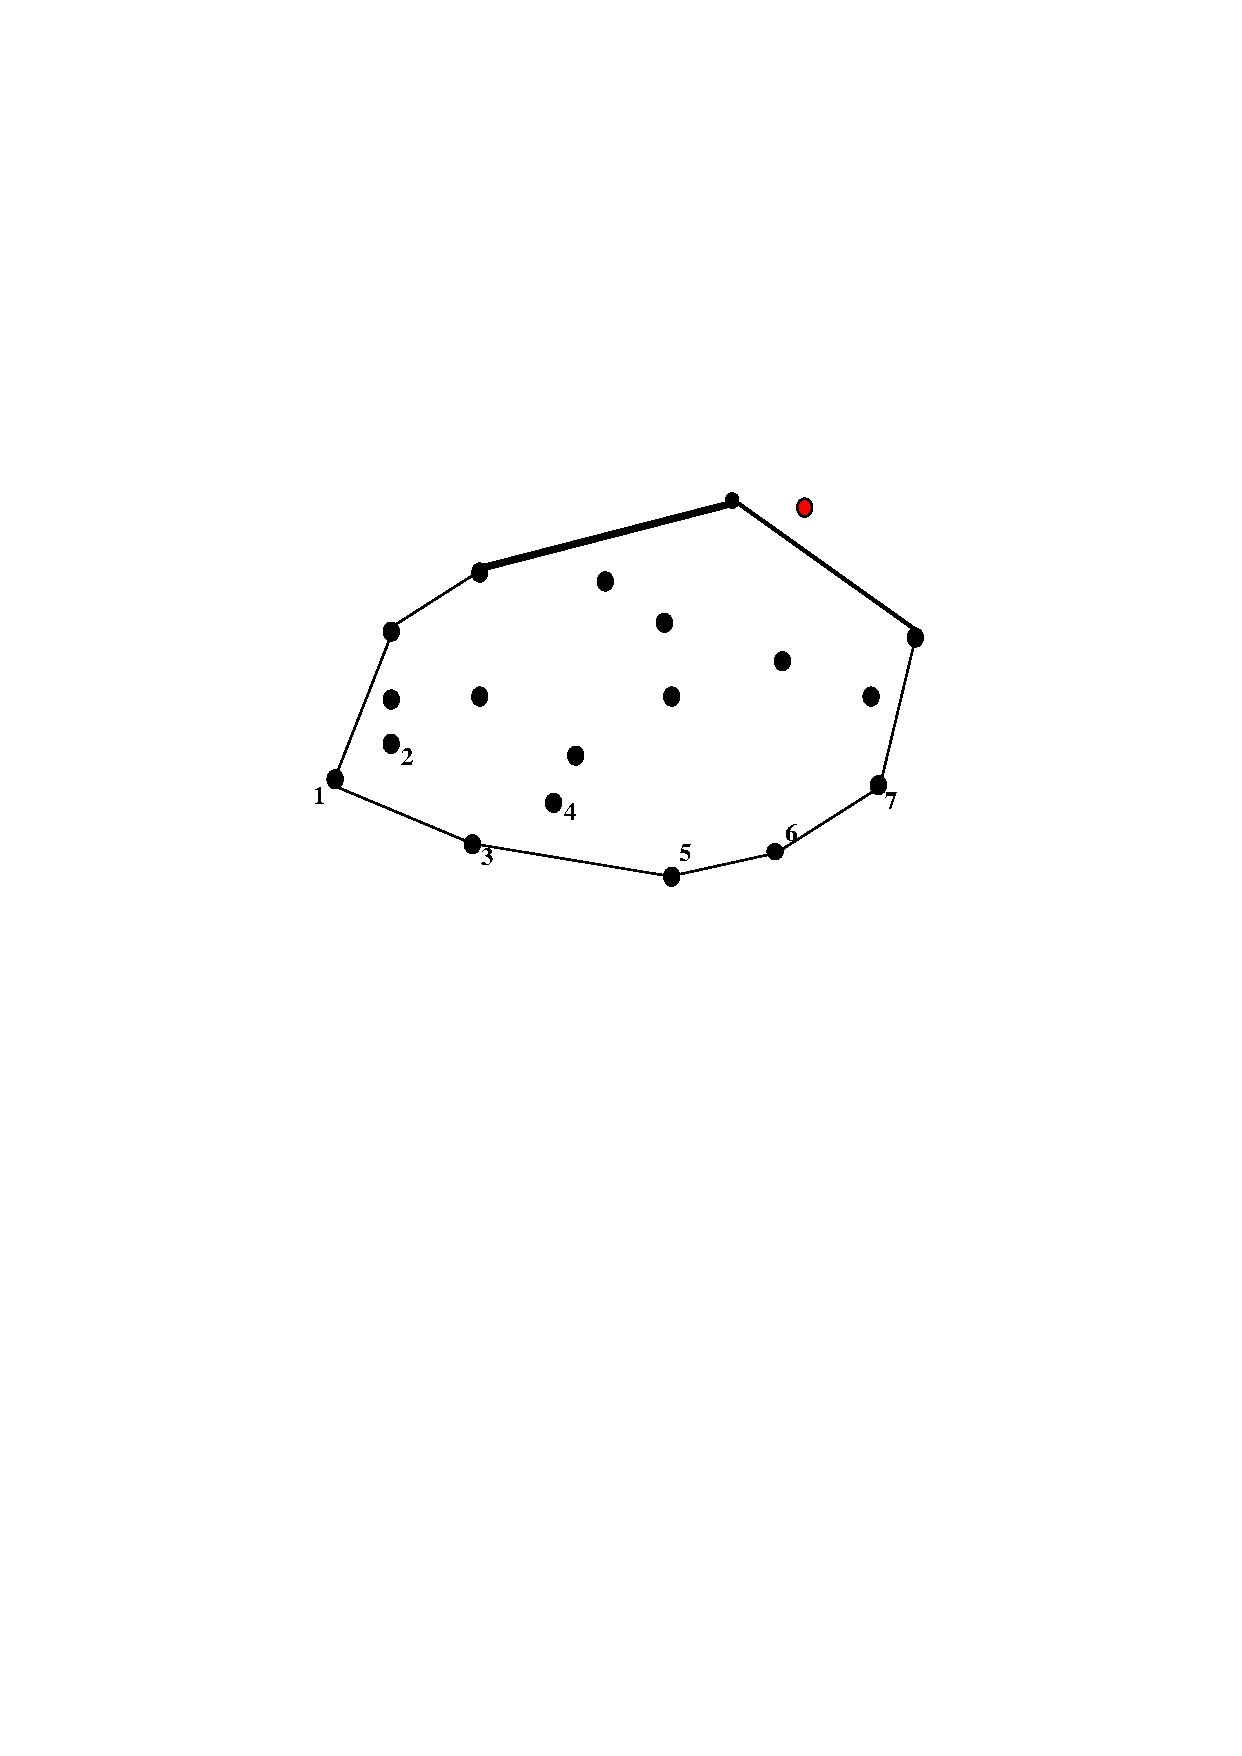
\includegraphics[width=0.28\textwidth]{figures/approximate-convexhull-step3.pdf}
        }
        \caption{二维近似内凸包的构造}
        \label{lbl:ach-2d}
        \end{figure}
        \vspace{-4mm}
        构造近似内凸包\footfullcite{bentley1982approximation},算法复杂度为~$O(n+\lambda)$,扩展到三维为~$O(n+\lambda^2 \log \lambda)$,然后利用$k$-means 聚类。
        
        \note{
          以二维为例,近似内凸包构造分为3个步骤,先分组,然后选出每组的极值点,最后将极值点按条件连接起来即可。此算法时间复杂度为~$O(n+\lambda)$,$\lambda$为分的组数。\\
          三维情况类似。\\
          得到近似凸包后,根据凸包面片的方向作为参与kmeans聚类算法的点集。
        }
    }
    \frame{
        \frametitle{$k$-means 聚类}
      \begin{figure}
        \vspace{-2mm}
        \subfloat[]
        {
           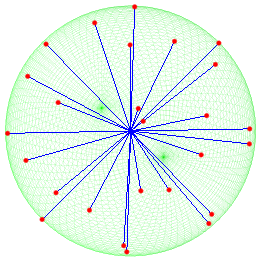
\includegraphics[width=0.25\textwidth]{kmeans-init-normals-26.png}
        }
        \subfloat[]
        {
            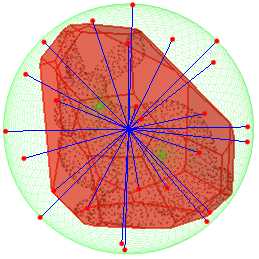
\includegraphics[width=0.25\textwidth]{kmeans-init-normals-26-for-bunny.png}
        }
        \subfloat[]
        {
           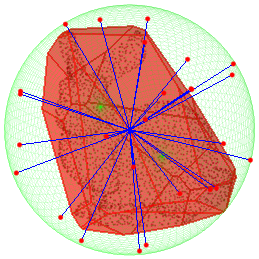
\includegraphics[width=0.25\textwidth]{kmeans-cluster-normals-26-for-bunny.png}
        }
        \vspace{-2mm}
        \caption{通过聚类确定法向}
        \label{lbl:gen-fixed-normals}
        \end{figure}
        \begin{description}
         \item[初始方向:]均匀分布;
         \item[距离度量:]余弦;
         \item[中心更新:]
   中心点:$\bm{c_i}=\frac{\sum_{i=1}^{i=n} \omega_i \cdot \bm{n_i} } {\sum_{i=1}^{i=n} \omega_i}$,权重$\omega_i$为面片面积。
        \end{description}

        \note{
          聚类算法需要关注下面3个问题,一是初始的方向,本文的算法采用均匀分布的方式确定,如图a,在球面上均匀分布k个点,球心和点的连线作为初始方向,图中k=26。 \\
          然后是类与类之间的距离如何度量,用余弦的方式可以使方向相近的点聚到一类。\\
          中心点的更新,以面片所在方向的面积作为权重,使得最后结果靠近面片较大的方向。图c为聚类后的结果,比图b紧致15\%左右。
        }
    }

  \subsection{搜索截面及求交}
    \frame{
    \frametitle{搜索截面}
    \begin{block}{截面=法向+点}
     法向已得,求投影点:对每个法向~$\bm{n_i}$,从输入模型的所有点中寻找最大投影值的点作为切点。
	时间复杂度为~$O(k\cdot n)$, 其中~$k$~为法向数量,$n$~为模型所含点数。
   \end{block}
   \begin{block}{并行可行性}
	各法向的计算相互独立, 借助~GPU~并行加速。
	典型GPU并行平台:着色器(GLSL为例)和基于 GPU 的通用计算框架(CUDA为例)。
	\end{block}

    \note{
     方向确定后,直接沿着方向搜索切点即可。因为各方向搜索过程相互独立,所以可借助GPU加速,本文采用两种典型的GPU加速平台,一种是OpenGL着色语言为代表的着色器平台,另一种是GPGPU通用计算框架CUDA。
    }
    }
    
    \frame{
    \frametitle{GLSL实现}
	     \begin{columns}[onlytextwidth]
     		 \begin{column}{0.5\textwidth}
		 \begin{figure}
	    		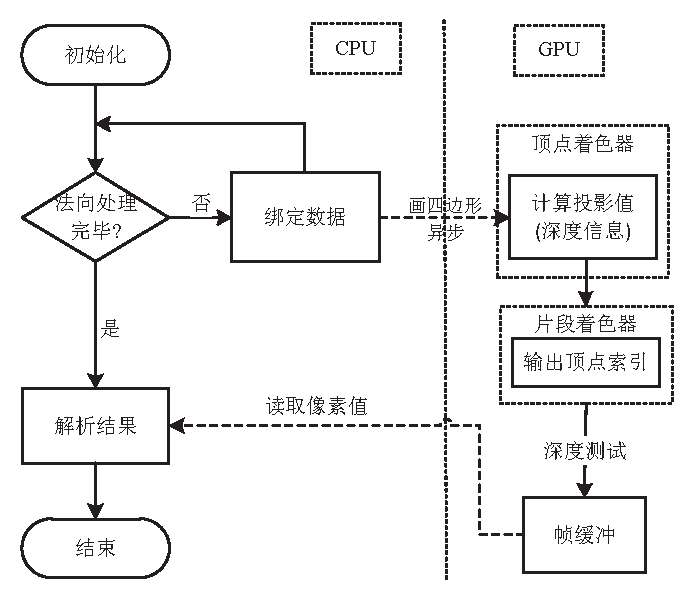
\includegraphics[width=\textwidth]{shader-z_buffer.eps}
	    		\caption{基于Z Buffer算法流程图}
		\end{figure}
	    	\end{column}
          \hspace{1em}
           \begin{column}{0.5\textwidth}
		   	\begin{figure}
		 	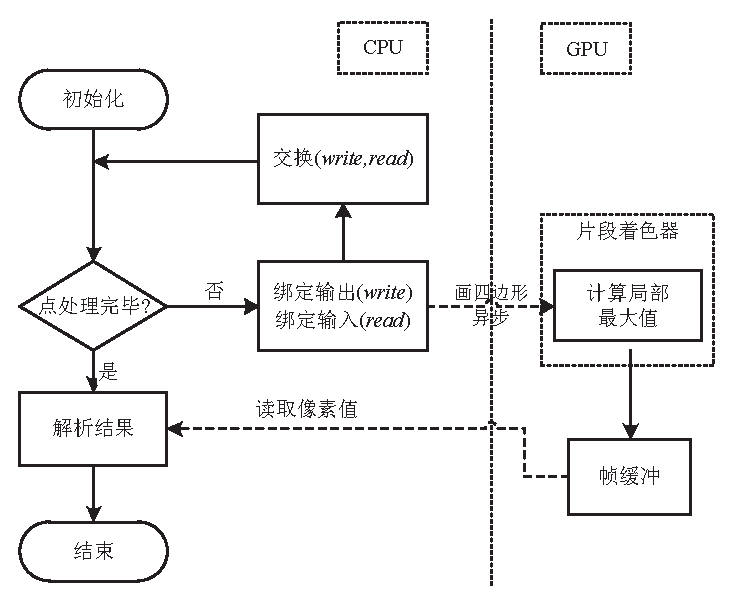
\includegraphics[width=\textwidth]{shader-rtt_pp.eps}
	    		\caption{基于乒乓技术算法流程图}
			\end{figure}	
	    	\end{column}
       	\end{columns}

        \note{
          \scriptsize
          GLSL中,本文提出了两种算法,
          一种是利用OpenGL的深度测试,深度测试实际上是比较三维点中z值的大小,在顶点着色器中,将所有点的 x,y 坐标值设为一样,并将该点在法向上的投影作为 z 值即深度值,所有点经过深度测试后将只有 z 值最大的点被保留下来,该点就是沿着这个法向的切点。这样经过k次渲染即可找到所有的k个切点。\\
          \scriptsize
          另外一种是乒乓技术,乒乓技术是需要把前一次运算结果传递给下一次运算用来作为后继运算的输。算法分批处理输入点集,每次计算能得到k个局部投影最大值,当所有点都被处理完毕后得到沿着所有法向投影最大值的点即切点。所以这个算法对k不是很敏感,因为k相对较小时,GPU一次总能处理k个方向,这点从后面的实验结果也能看出。
        }
   }
    
    \begin{frame}
    \frametitle{CUDA实现}
    \vspace{-1em}
	    \begin{figure}
	    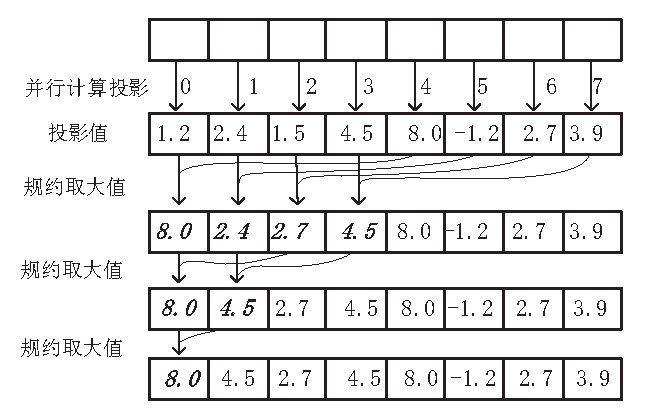
\includegraphics[width=2.5in]{gpureduction.eps}
	    \caption{并行规约求最大投影值}
	    \label{lbl:reduction-getmax}
	    \end{figure}
	    \vspace{-1.5em}
	    \small 
	    将输入点交给数量为~$t$~的线程计算点积得到投影值,
 线程~$i$~和~$i+t/2$~比较选取较大者,经~$\log_2t$~次比较可得最大值。OpenCL等并行计算框架类似。
  
 \note{
      CUDA实现中原理如上图所示,将输入点交给数量为~$t$~的线程计算点积得到投影值,线程~$i$~和~$i+t/2$~比较选取较大者,经~$\log_2t$~次比较可得最大值。
      这种规约方式在其他GPGPU框架中也类似,如OpenCL等。
 }
    \end{frame}

        \frame{
    \frametitle{求交算法}
      \begin{block}{直接枚举}
      通过枚举所有每~3~个平面交于~1~点的情况,然后排除在平面外部的交点,剩下的构成~$k$-CBP~的顶点,时间复杂度为$O(k^3)$。
      \end{block}
      \begin{block}{对偶映射}
        法向~$\bm{n}(a,b,c)$~ + 平面上点~$\bm{p}(x_0,y_0,z_0)$ $\Rightarrow$ 平面方程~$ax + by + cz = ax_0 + by_0 + cz_0=d$, $d \neq 0$ \\
        对偶点为~$\bm{p'}(a/d, b/d, c/d)$,对~$k$~个映射点求凸包,凸包平面映射回原来的交点,时间复杂度为$O(k\log k)$。\footfullcite{dengcg}
      \end{block}
      
      \note{
        确定平面后,接下来就是求每个平面上的交点。一种比较直接的算法是通过枚举所有每~3~个平面交于~1~点的情况,然后排除在平面外部的交点,剩下的构成~$k$-CBP~的顶点,时间复杂度为$O(k^3)$。
        通过计算几何中的对偶映射技术可以将复杂度降低到$O(k\log k)$。
      }
    }

  \subsection{实验结果与分析}

  %\subsubsection{凸包围多面体的生成速度}

    \frame{
      \frametitle{生成$k$-CBP的效率:GLSL实验结果}
      \vspace{-1em}
      \begin{figure}[htbp] % use [htbp] to fix the position
      \vspace{-8mm}
      \subfloat %Apple模型(8118个点)
      {  
         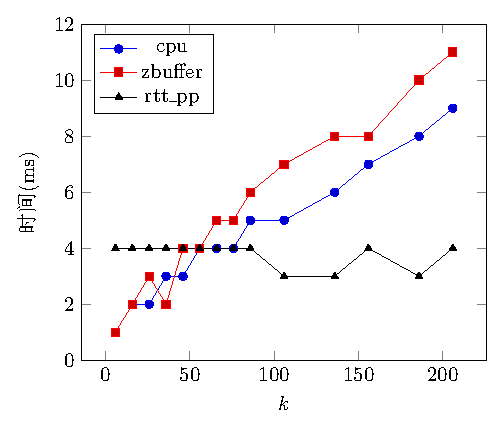
\includegraphics[width=\fourgraphicswidth\textwidth,page=1]{shadertime.pdf}
      }
      \subfloat % Buddha模型(31232个点)
      {  
          \includegraphics[width=\fourgraphicswidth\textwidth, page=2]{shadertime.pdf}
      }\vspace{-8mm}\linebreak %强制换行
        \vspace{-3mm}%
      \subfloat % Alice模型(224291个点)
      {  
         \includegraphics[width=\fourgraphicswidth\textwidth, page=3]{shadertime.pdf}
      }
      \subfloat % Bugatti模型(1010815个点)
      {  
         \includegraphics[width=\fourgraphicswidth\textwidth, page=4]{shadertime.pdf}
      }
      \caption{\tiny Apple(8k), Buddha(31k), Alice(224k), Bugatti(1011k)}
      \label{fig:chart:exps:shadertime}
      \end{figure}

      \note{
        这是基于OpenGL着色语言实现的实验结果。
      从实验结果可以看出,当模型规模不大时,如左上图所示的含有8千多个点的~Apple~模型,
Z Buffer~算法和传统的~CPU~算法差别不是很大,因此在实际应用中当模型规模较小时可直接用~CPU~计算即可。
随着输入模型所含有点的数量规模的增加,CPU~和~GPU~运行时间之间的差距也越来越大。
当多面体面数增加即~$k$~的增大时,在~Z Buffer~算法中,需要更多的绘制次数,因此其运行时间也有所增加,而在基于乒乓技术的算法中,当点规模一定时,$k$~的变化对最后运行时间影响不明显,因此当较大的~$k$~时,这种算法更快。
      }
    }

    \frame{
      \frametitle{生成$k$-CBP的效率:CUDA实验结果}
      \vspace{-1em}
        \begin{figure}
        \vspace{-8mm}
        \subfloat%[\tiny Budda(31232 points)]
        { 
           \includegraphics[width=0.35\textwidth,page=2]{figures/cudatime.pdf}
        }
        \subfloat%[\tiny Dinosaur(40277 points)]
        { 
            \includegraphics[width=0.35\textwidth, page=3]{figures/cudatime.pdf}
        }\vspace{-8mm}\linebreak %强制换行
        \vspace{-3mm}%
       \subfloat%[Alice(224291 points)]
        {
           \includegraphics[width=0.35\textwidth, page=4]{figures/cudatime.pdf}
        }
        \subfloat%[Bugatti(1010815 points)]
        {
           \includegraphics[width=0.35\textwidth, page=5]{figures/cudatime.pdf}
        }
        \caption{\tiny Budda(31k),Dinosaur(40k),Alice(224k), Bugatti(1011k)}
        \label{chart:exps:cputime}
        \end{figure}

        \note{
         这是CUDA的实验结果,
        图中横纵坐标分别代表多面体面数和运行时间, 其中虚线代表搜索截面的过程, 实线为构造凸包围多面体总体耗时. 当模型点数量较大时, 搜索截面的过程占据了算法绝大多数时间, 且随着凸包围多面体的面数~$k$~ 值增加而线性增长, 这与搜索截面时间复杂度($O(k\cdot n)$)一致, 截面求交过程的时间复杂度为$O(k\log k)$,
当点数量极大时, 实线虚线几乎重合即求交等步骤耗时相比整体算法而言几乎可忽略.
        }
    }

    \frame{
      \frametitle{生成$k$-CBP的效率:与文献\cite{karlsson2010parallel}算法对比}
        \vspace{-7mm}
        \begin{table} \tiny
          \caption{本文算法与文献\footfullcite{karlsson2010parallel}算法对比}
        \begin{tabular}{p{1.5cm}<{\centering}ccc ccc} %p本身占一列
       \toprule[1pt]
        \multirow{2}{*}{$k$} & \multicolumn{3}{c}{Apple(8118 points)} & \multicolumn{3}{c}{~~~~~Bugatti(1010815 points)}\\
        ~&文献\cite{karlsson2010parallel}(ms) & $k$-CBP(ms) &  Speedup &文献\cite{karlsson2010parallel}(ms) & $k$-CBP(ms) &  Speedup \\
     \midrule[0.5pt]
        6 & 0.4 & 0.12  & 3.20     & 24.2 & 3.20  & 7.56 \\
        16 & 0.9 & 0.26  & 3.43    & 44.5 & 8.44  & 5.27 \\
        26 & 1.4 & 0.41  & 3.38    & 66.5 & 13.65  & 4.87 \\
        36 & 1.9 & 0.52  & 3.65    & 91.1 & 18.34  & 4.97 \\
        46 & 2.5 & 0.67  & 3.74    & 119.5 & 24.13  & 4.95 \\
        56 & 2.9 & 0.79  & 3.66    & 138.4 & 28.86  & 4.80 \\
        66 & 3.5 & 0.95  & 3.69    & 170.6 & 34.10  & 5.00 \\
        76 & 4.0 & 1.08  & 3.70      & 197.1 & 39.85  & 4.95 \\
        86 & 4.5 & 1.22  & 3.69    & 219.8 & 45.08  & 4.88 \\
        106 & 5.4 & 1.49  & 3.62   & 267.8 & 55.52  & 4.82 \\
        136 &  6.8 & 1.92  & 3.54  & 342.9 & 71.24  & 4.81 \\
        156 &  7.7 & 2.17  & 3.55  & 411.3 & 81.18  & 5.07 \\
        186 &  9.3 & 2.60  & 3.58  & 479.4 & 97.39  & 4.92 \\
        206 &  10.5 & 2.85  & 3.68 & 523.0 & 106.87  & 4.89  \\  
        \bottomrule[1pt]
        \end{tabular}
        \label{tab:exp:sse-time}
        \end{table}
        \vspace{-3mm}
        \scriptsize  当点数量较小时,能够提高~3-4~倍速度,模型变大,加速比更大,Bugatti~模型的提速达到~4$\sim$8~倍。
        
        \note{
         这是和一篇专门讲并行求包围体的算法的论文的对比结果(Swedish瑞典,sigrad会是Eurographics的子会议议题官网说的是the Swedish Chapter of Eurographics),可以看出当点数量较小时,能够提高~3-4~倍速度,模型变大,加速比更大,Bugatti~模型的提速达到~4$\sim$8~倍。
        }
    }

  %\subsubsection{凸包围多面体的紧致程度}
   \frame{
        \frametitle{生成$k$-CBP的紧致程度:$k$-DOP v.s $k$-CBP }
        \begin{figure}
        \vspace{-8mm}
        \subfloat
        {  
           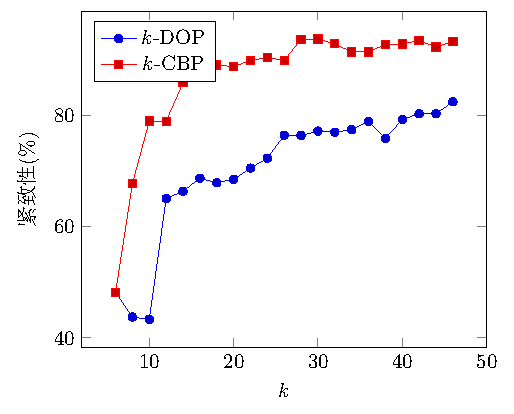
\includegraphics[width=0.35\textwidth,page=1]{figures/tightness.pdf}
        }
        \subfloat
        { 
            \includegraphics[width=0.35\textwidth, page=2]{figures/tightness.pdf}
        }\vspace{-8mm}\linebreak %强制换行
        \vspace{-3mm}%
       \subfloat%[Alice(224291 points)]
        { 
           \includegraphics[width=0.35\textwidth, page=3]{figures/tightness.pdf}
        }
        \subfloat%[Bugatti(1010815 points)]
        {
           \includegraphics[width=0.35\textwidth, page=4]{figures/tightness.pdf}
        }
        \caption{紧致程度对比: \tiny Apple(8k), Budda(31k), Dinosaur(40k), Alice(224k)}
        \label{chart:exps:tightness}
        \end{figure}
        
        \note{
          这是本文算法和k-DOP的对比,较~$k$-DOP~提升 10\% $\sim$ 40\%,下图可视化结果。
        }
    }
    \frame{
      \frametitle{生成$k$-CBP的紧致程度:$k$-DOP v.s $k$-CBP }
      \hspace{3em}
      \vspace{-3em}
      \begin{figure}[H] 
        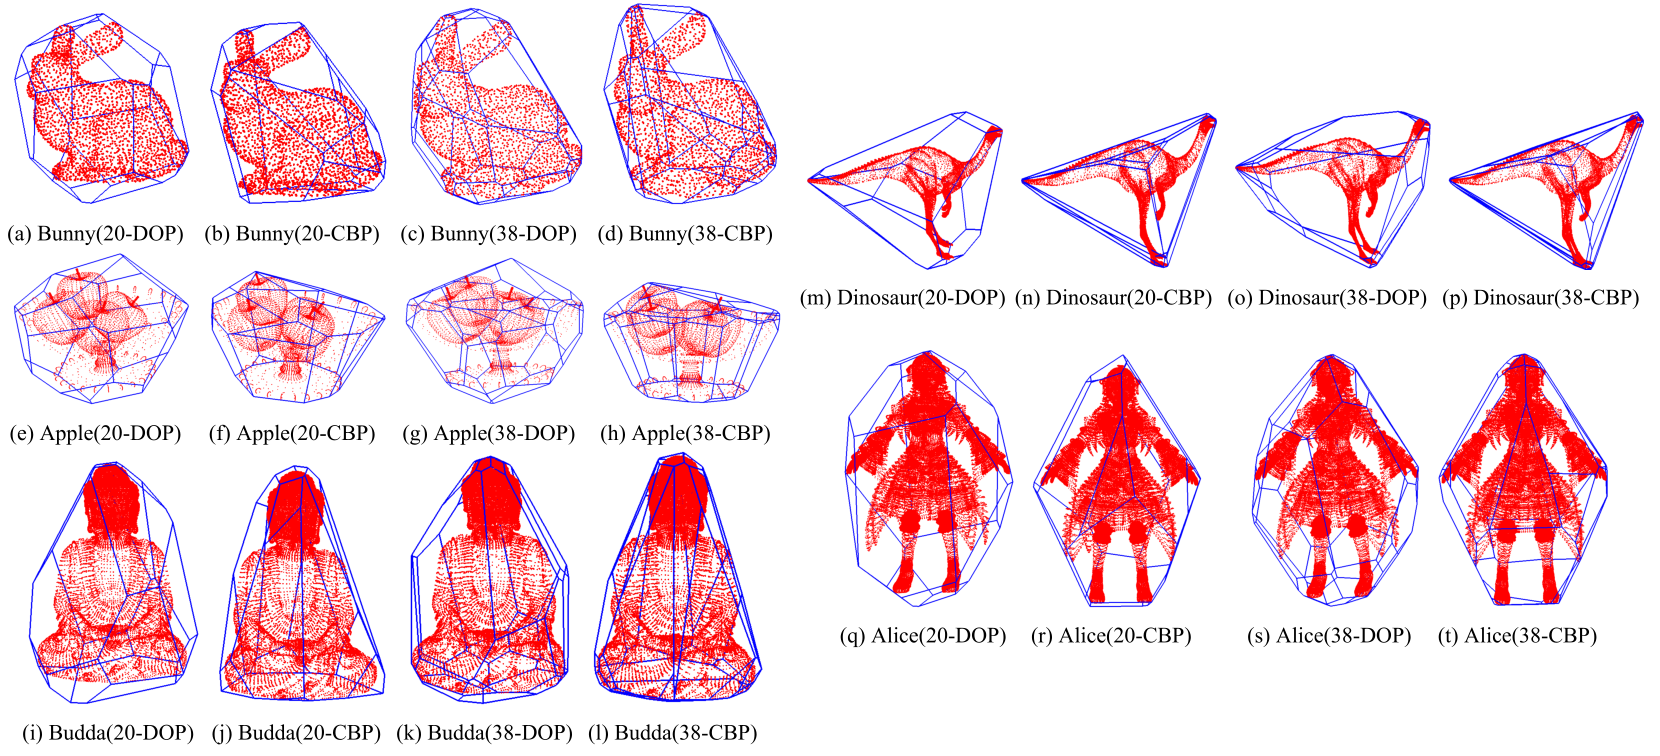
\includegraphics[width=1.05\textwidth]{kCBP-KDOP.png}
      \caption{~$k$-CBP~与~$k$-DOP~对比}
      \label{fig:kdop:kcbp:ui}
      \end{figure}

      \note{
        该图中是不同k值的对比,左边为k-DOP结果,右边为本文结果。从外观上看,确实也紧致了不少。
      }
    }

    \frame{
        \frametitle{生成$k$-CBP的紧致程度:$k$-CBP v.s 凸包 }
        \vspace{-2em}
        \begin{table}
        \scriptsize
        \caption{\label{tab:exp:cgal}$k$-CBP~与~QuickHull~凸包算法比较}
         \begin{tabular}{lcccccl}
          \toprule
          Model & f(CHull)& f($k$-CBP) & $\tau$ ($k$-CBP) & t(CHull(ms)) & t($k$-CBP(ms))\\
          \midrule
          Apple	& 499 & 30 & 93.67\% & 5.5 & 1.30\\ % apple3  自己电脑跑的数据, 之前是用的chengxianyu的电脑.
          Budda	& 1608 & 46 & 92.39\% & 21.3 & 2.86 \\ %  1.0+0.86+1
          Dinosaur	& 1240 & 44 & 93.34\% & 22.6 & 1.99 \\  % 1.0+0.98+0.1
          Alice	& 1332 & 44 & 93.92\% & 85.8 & 8.47\\ % 2+6.48
          Bugatti & 24654 & 44 & 95.06\% & 688.7 & 25.41\\
          \bottomrule
         \end{tabular}
         \vspace{-2mm}
        \end{table}
        \begin{block}{结论}
        \footnotesize 与凸包相比,本文算法在大大简化包围体平面数量的同时能保持较好的紧致程度(Bugatti 凸包面的0.17\%的达到95.06\%紧致程度,构造速度快27倍),下图为可视化结果。
        \end{block}

        \note{
        这是本文算法和CGAL中的凸包的对比,其中f表示面数量,$\tau$的值为紧致程度,紧致程度是用凸包的体积除以凸包围多面体的体积来衡量的。与凸包相比,本文算法在大大简化包围体平面数量的同时能保持较好的紧致程度(Bugatti 凸包面的0.17\%的达到95.06\%紧致程度,构造速度快27倍),下图为可视化结果。
      }
    }

    \frame{
        \frametitle{生成$k$-CBP的紧致程度:$k$-CBP v.s 凸包}
        \begin{figure}
        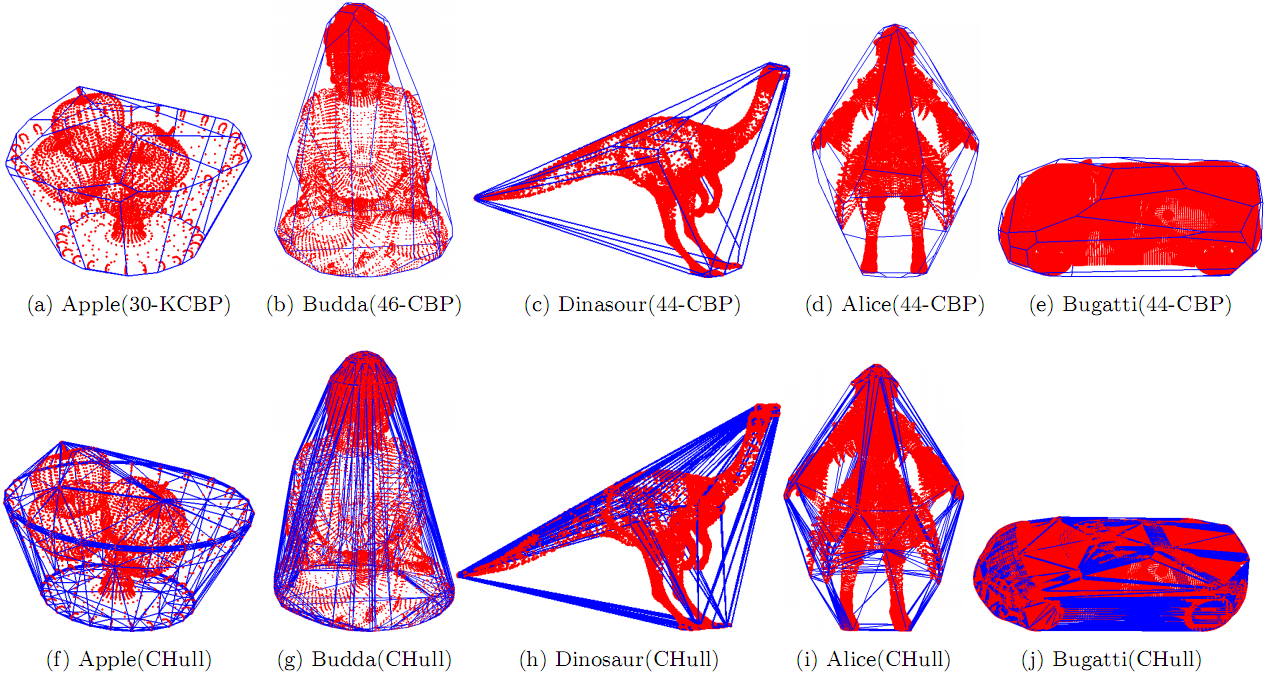
\includegraphics[width=4.0in]{figures/kcbp-convexhull.png}
        \caption{$k$-CBP~与凸包对比}
        \label{pic:exps:ch-kcbp}
        \end{figure}
    }
